\documentclass[11pt,a4paper]{article}
\usepackage[utf8]{inputenc}
\usepackage[T1]{fontenc}
\usepackage{lmodern}
\usepackage[margin=2.2cm]{geometry}
\usepackage{amsmath,amssymb}
\usepackage{graphicx}
\usepackage{booktabs}
\usepackage{float}
\usepackage{caption}
\usepackage[hidelinks]{hyperref}
\usepackage{xurl}

\renewcommand{\figurename}{Figura}
\renewcommand{\tablename}{Tabla}
\renewcommand{\refname}{Referencias}
\newcommand{\sen}{\operatorname{sen}}
% \input primitivo: se puede usar dentro de un tabular
\makeatletter\newcommand{\filasTabla}[1]{\@@input #1 }\makeatother
\captionsetup{font=small,labelsep=colon}
\setlength{\parindent}{0pt}
\setlength{\parskip}{5pt}

% Generado por main.py - no editar a mano
\newcommand{\vLmm}{250}
\newcommand{\vrmm}{20}
\newcommand{\vemm}{150}
\newcommand{\vTman}{3.0}
\newcommand{\vtest}{1.217}
\newcommand{\vwest}{3.193}
\newcommand{\vaest}{2.043}
\newcommand{\vxAest}{204.8}
\newcommand{\vyAest}{143.4}
\newcommand{\vxPest}{354.8}
\newcommand{\vvAxest}{-0.458}
\newcommand{\vvAyest}{0.654}
\newcommand{\vvAest}{0.798}
\newcommand{\vatest}{0.511}
\newcommand{\vanest}{2.548}
\newcommand{\vaAxest}{-2.380}
\newcommand{\vaAyest}{-1.043}
\newcommand{\vaAest}{2.599}
\newcommand{\vwmax}{3.491}
\newcommand{\vamax}{3.655}
\newcommand{\vvPmax}{0.873}
\newcommand{\vaPmax}{3.046}


\begin{document}

\begin{center}
{\Large\textbf{Escuela Superior Politécnica del Litoral}}\\[2pt]
Mecánica de Maquinaria -- PAO II 2026\\[8pt]
{\large\textbf{AVANCE 3: ANÁLISIS CINEMÁTICO}}\\[6pt]
Diego Pontón -- Joshua Vélez\\
Profesor: Livinston Castro
\end{center}

\section{Mecanismo y datos}

El mecanismo es el brazo con gripper paralelo al suelo del Avance 2: un cuatro barras en
paralelogramo en el que la correa, con poleas iguales, reemplaza a la barra superior. Los
eslabones son: 1, bancada (chasis y polea trasera fija); 2, brazo; 3, polea delantera unida al
gripper; y 4, barra virtual (correa). Tiene un grado de libertad ($M=1$) y cumple $s+l=p+q$
(caso especial de Grashof), por lo que el brazo puede girar de forma continua.

El origen está en el eje de la polea trasera $O_2$, con $x$ hacia delante y $y$ hacia arriba. Los
ángulos se miden desde $+x$ en sentido antihorario. La entrada es el ángulo del brazo $\theta_2$.

\begin{table}[H]
\centering
\caption{Datos del mecanismo (plano del Avance 2).}
\label{tab:datos}
\small
\begin{tabular}{@{}lll@{}}
\toprule
Símbolo & Descripción & Valor \\
\midrule
$L$ & Distancia entre ejes de las poleas (brazo y correa) & \vLmm\ mm \\
$d=r$ & Radio de las poleas (bancada y acoplador del paralelogramo) & \vrmm\ mm \\
$e$ & Eje delantero a la punta de los dedos ($P$) & \vemm\ mm \\
$\theta_1$ & Orientación de la bancada $O_2O_4$ & $90^\circ$ \\
$\theta_2$ & Rango de trabajo del brazo & $-60^\circ$ a $240^\circ$ ($300^\circ$) \\
\bottomrule
\end{tabular}
\end{table}

\section{Análisis de posición}

La ecuación de lazo y sus componentes son:
\begin{gather}
\mathbf{r}_2+\mathbf{r}_3=\mathbf{r}_1+\mathbf{r}_4,\\
L\cos\theta_2+d\cos\theta_3=d\cos\theta_1+L\cos\theta_4,\qquad
L\sen\theta_2+d\sen\theta_3=d\sen\theta_1+L\sen\theta_4.
\end{gather}
Para saber qué solución toma el mecanismo se usa la relación de la transmisión por banda. Con
el brazo como referencia, como en un tren epicíclico, y con poleas iguales:
\begin{equation}
\frac{\omega_3-\omega_2}{\omega_1-\omega_2}=\frac{r_1}{r_3}=1
\quad\Rightarrow\quad \omega_3=\omega_1=0.
\label{eq:banda}
\end{equation}
La polea delantera no gira, así que $\theta_3$ se mantiene constante en $90^\circ$. Al reemplazar en
el lazo se obtiene
\begin{equation}
\theta_3=90^\circ,\qquad \theta_4=\theta_2.
\end{equation}
El gripper queda paralelo al suelo en cualquier posición del brazo. La posición de los puntos de
interés es:
\begin{equation}
\mathbf{r}_A=L\,(\cos\theta_2,\ \sen\theta_2),\qquad
\mathbf{r}_P=\mathbf{r}_A+(e,\ 0),\qquad
\mathbf{r}_{G_2}=\tfrac12\,\mathbf{r}_A,
\end{equation}
donde $A$ es el centro de la polea delantera, $P$ la punta de los dedos y $G_2$ el centro de masa
del brazo. La punta del gripper recorre una circunferencia de radio $L$ centrada en $(e,0)$
(Figura~\ref{fig:tray}).

\begin{figure}[H]
\centering
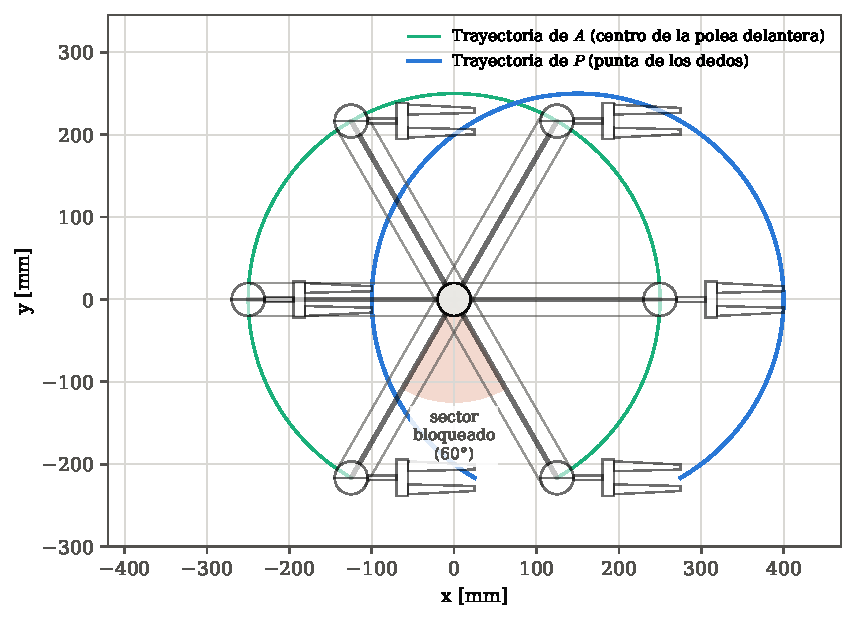
\includegraphics[width=0.62\textwidth]{../figuras/fig_trayectoria}
\caption{Trayectorias de $A$ y $P$, con el mecanismo dibujado cada $60^\circ$. El gripper no
cambia de orientación.}
\label{fig:tray}
\end{figure}

\section{Análisis de velocidad}

Se usa la ecuación de velocidad relativa entre dos puntos de un mismo eslabón,
$\mathbf{v}_B=\mathbf{v}_A+\boldsymbol{\omega}\times\mathbf{r}_{B/A}$. Para el punto $A$ del brazo:
\begin{equation}
\mathbf{v}_A=\omega_2\,\hat{k}\times\mathbf{r}_{A/O_2}=L\,\omega_2\,(-\sen\theta_2,\ \cos\theta_2).
\end{equation}
El punto $B$ (sobre la polea delantera, a una distancia $d$ de $A$) se puede escribir desde la
barra 4 o desde el acoplador 3:
\begin{equation}
\omega_4\,\hat{k}\times\mathbf{r}_{B/O_4}=\mathbf{v}_A+\omega_3\,\hat{k}\times\mathbf{r}_{B/A}.
\end{equation}
Con $\theta_3=90^\circ$ y $\theta_4=\theta_2$, sus componentes son:
\begin{align}
x:&\quad -L\omega_4\sen\theta_2=-L\omega_2\sen\theta_2-d\,\omega_3,\\
y:&\quad \phantom{-}L\omega_4\cos\theta_2=L\omega_2\cos\theta_2.
\end{align}
De la ecuación en $y$ se obtiene $\omega_4=\omega_2$, y al reemplazarla en la ecuación en $x$,
$\omega_3=0$, lo que coincide con la ecuación~\eqref{eq:banda}. Cuando el brazo está vertical
($\theta_2=90^\circ$), la ecuación en $y$ no define $\omega_4$; un paralelogramo de barras rígidas
podría cruzarse en esa posición. Con la correa, $\omega_3=0$ siempre, y la ecuación en $x$ da
$\omega_4=\omega_2$.

Como el gripper no rota ($\omega_3=0$), todos sus puntos tienen la velocidad de $A$:
\begin{equation}
\mathbf{v}_P=\mathbf{v}_A+\omega_3\,\hat{k}\times\mathbf{r}_{P/A}=\mathbf{v}_A,\qquad
|\mathbf{v}_P|=L\,|\omega_2|,\qquad \mathbf{v}_{G_2}=\tfrac12\,\mathbf{v}_A.
\end{equation}

\section{Análisis de aceleración}

Para dos puntos de un mismo eslabón,
$\mathbf{a}_B=\mathbf{a}_A+\boldsymbol{\alpha}\times\mathbf{r}_{B/A}-\omega^2\,\mathbf{r}_{B/A}$. No
hay deslizamiento entre eslabones, por lo que no aparece el término de Coriolis. Para $A$:
\begin{equation}
\mathbf{a}_A=\underbrace{L\,\alpha_2\,(-\sen\theta_2,\ \cos\theta_2)}_{\text{tangencial},\ a^t=L\alpha_2}
+\underbrace{L\,\omega_2^2\,(-\cos\theta_2,\ -\sen\theta_2)}_{\text{normal},\ a^n=L\omega_2^2},
\qquad |\mathbf{a}_A|=L\sqrt{\alpha_2^2+\omega_2^4}.
\end{equation}
Al escribir $\mathbf{a}_B$ desde la barra 4 y desde el acoplador, con $\omega_3=0$ y
$\omega_4=\omega_2$:
\begin{align}
x:&\quad -L\alpha_4\sen\theta_2-L\omega_2^2\cos\theta_2=-L\alpha_2\sen\theta_2-L\omega_2^2\cos\theta_2-d\,\alpha_3,\\
y:&\quad \phantom{-}L\alpha_4\cos\theta_2-L\omega_2^2\sen\theta_2=L\alpha_2\cos\theta_2-L\omega_2^2\sen\theta_2,
\end{align}
de donde $\alpha_4=\alpha_2$ y $\alpha_3=0$. Entonces todo el gripper tiene la aceleración de $A$:
\begin{equation}
\mathbf{a}_P=\mathbf{a}_A,\qquad \mathbf{a}_{G_2}=\tfrac12\,\mathbf{a}_A.
\end{equation}

\section{Resultados numéricos}

Como el actuador se define en el Avance 4, se supone que el brazo recorre los $300^\circ$ en
$T=\vTman$~s con una ley cicloidal, que arranca y se detiene con velocidad y aceleración nulas:
\begin{equation}
\theta_2=\theta_{2,0}+\Delta\theta\left[\frac{t}{T}-\frac{1}{2\pi}\sen\frac{2\pi t}{T}\right],\quad
\omega_2=\frac{\Delta\theta}{T}\left[1-\cos\frac{2\pi t}{T}\right],\quad
\alpha_2=\frac{2\pi\Delta\theta}{T^2}\sen\frac{2\pi t}{T},
\end{equation}
con $\theta_{2,0}=-60^\circ$ y $\Delta\theta=300^\circ$.

\textbf{Posición de estudio, $\theta_2=35^\circ$} (la de la vista lateral del Avance 2). El brazo pasa
por ella en $t=\vtest$~s, con $\omega_2=\vwest$~rad/s y $\alpha_2=\vaest$~rad/s$^2$:
\begin{align*}
\mathbf{r}_A&=250\,(\cos35^\circ,\ \sen35^\circ)=(\vxAest,\ \vyAest)~\text{mm},\qquad
\mathbf{r}_P=(\vxPest,\ \vyAest)~\text{mm},\\
\mathbf{v}_P&=\mathbf{v}_A=(0.250)(\vwest)(-\sen35^\circ,\ \cos35^\circ)=(\vvAxest,\ \vvAyest)~\text{m/s},
\qquad |\mathbf{v}_P|=\vvAest~\text{m/s},\\
a^t&=(0.250)(\vaest)=\vatest~\text{m/s}^2,\qquad a^n=(0.250)(\vwest)^2=\vanest~\text{m/s}^2,\\
\mathbf{a}_P&=\mathbf{a}_A=(\vaAxest,\ \vaAyest)~\text{m/s}^2,\qquad |\mathbf{a}_P|=\vaAest~\text{m/s}^2,\\
\omega_3&=\alpha_3=0,\qquad \omega_4=\vwest~\text{rad/s},\qquad \alpha_4=\vaest~\text{rad/s}^2.
\end{align*}

\begin{figure}[H]
\centering
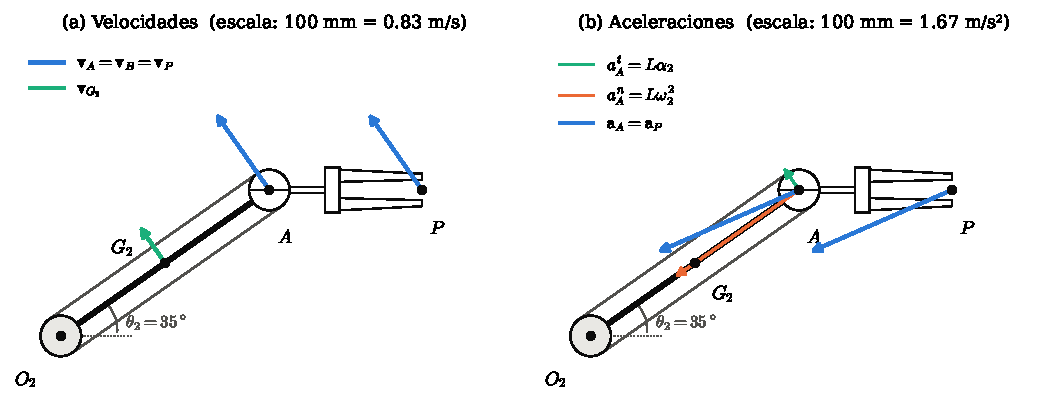
\includegraphics[width=0.95\textwidth]{../figuras/fig_estado35}
\caption{Velocidades y aceleraciones en $\theta_2=35^\circ$, dibujadas a escala.}
\label{fig:est}
\end{figure}

\textbf{Todo el recorrido.} Con scripts en Python se evaluaron las ecuaciones en toda la
maniobra (Tabla~\ref{tab:res} y Figura~\ref{fig:grip}). Los scripts de todos los cálculos y
gráficas de este avance están en el repositorio:
\begin{center}\footnotesize\url{https://github.com/diegoPonton/scripts-de-calculos-y-gr-ficas-mecanica-de-maquinaria-proyecto}\end{center}
Los máximos ocurren con el brazo vertical
($\theta_2=90^\circ$, $t=1.5$~s): $\omega_2=\vwmax$~rad/s, $|\mathbf{v}_P|=\vvPmax$~m/s y
$|\mathbf{a}_P|=\vaPmax$~m/s$^2$. La aceleración angular máxima es $\alpha_2=\vamax$~rad/s$^2$.

\begin{table}[H]
\centering
\caption{Resultados cada $30^\circ$ ($\theta_3=90^\circ$, $\theta_4=\theta_2$,
$\omega_3=\alpha_3=0$, $\omega_4=\omega_2$ y $\alpha_4=\alpha_2$ en todas las filas).}
\label{tab:res}
\small
\begin{tabular}{@{}rrrrrrrr@{}}
\toprule
$\theta_2$ [°] & $t$ [s] & $x_P$ [mm] & $y_P$ [mm] & $\omega_2$ [rad/s] & $\alpha_2$ [rad/s$^2$] &
$|\mathbf{v}_P|$ [m/s] & $|\mathbf{a}_P|$ [m/s$^2$] \\
\midrule
\filasTabla{../resultados/tabla_resultados.tex}
\bottomrule
\end{tabular}
\end{table}

\begin{figure}[H]
\centering
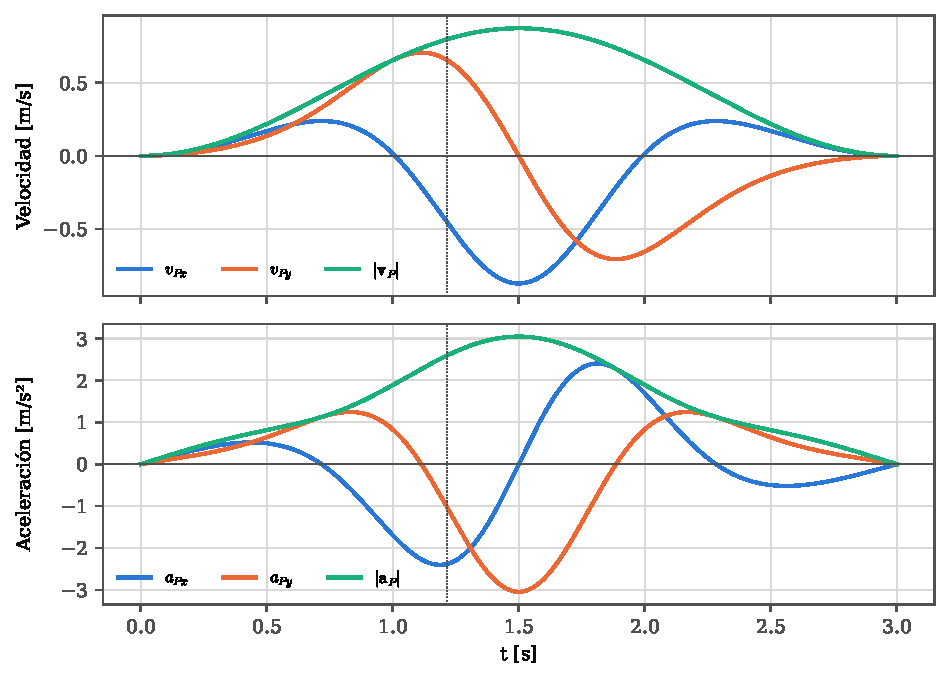
\includegraphics[width=0.72\textwidth]{../figuras/fig_gripper}
\caption{Velocidad y aceleración de la punta del gripper durante la maniobra. La línea punteada
marca $\theta_2=35^\circ$.}
\label{fig:grip}
\end{figure}

\section{Conclusiones}

\begin{itemize}
\item Con poleas iguales y la polea trasera fija, la polea delantera no gira: $\theta_3=90^\circ$,
$\omega_3=\alpha_3=0$. El gripper se mantiene paralelo al suelo en todo el recorrido.
\item El brazo y la correa giran juntos: $\theta_4=\theta_2$, $\omega_4=\omega_2$ y
$\alpha_4=\alpha_2$.
\item Todo el gripper tiene la velocidad y la aceleración del centro de la polea delantera, con
máximos de \vvPmax~m/s y \vaPmax~m/s$^2$. Estos valores se usarán en el análisis dinámico del
Avance 4.
\end{itemize}

\end{document}
